\documentclass[a4paper, 10pt]{article}
\usepackage{fullpage}
\usepackage{titling}
\usepackage{graphics}
\usepackage{amsmath}
\usepackage{amssymb}
\usepackage{hyperref}
\usepackage{IEEEtrantools}
\usepackage{graphicx}
\usepackage{tcolorbox}
\usepackage{xcolor}
\usepackage[normalem]{ulem}

\setlength{\droptitle}{-6em}   % This is your set screw, for shifting up the title
\renewcommand{\baselinestretch}{1.1}
\setlength{\parskip}{0.5em}

\author{}
\date{}
\title{Worksheet 8 \vspace{-0.5cm}}

\DeclareMathOperator{\E}{\mathbb{E}}
\DeclareMathOperator{\V}{\mathbb{V}}

\begin{document}
\maketitle
\vspace{-2cm}

\subsubsection*{Q1}
(\textit{Exercise 6.11 S\&B})
Why is Q-learning considered an off-policy control method?

\subsubsection*{Answer:}
Q--learning learns the state--action value function for the optimal (greedy) policy while its trajectory is generated under the exploratory policy (such as the $\epsilon$--greedy policy). We can see this from the Q learning update equation which differs from the SARSA update equation, by including a max operator over the next state action Q values instead of using $Q(S', A')$ sampled from the exploratory policy. As a result, the action values are learned for the greedy policy.

\subsubsection*{Q2}
(\textit{Exercise 6.12 S\&B})
Suppose action selection is greedy. Is Q-learning then exactly the same
algorithm as Sarsa? Will they make exactly the same action selections and weight
updates? (\textbf{Additional Challenge:} What about Expected Sarsa? Does it have the same or different updates as Q-learning or Sarsa?)

\subsubsection*{Answer:}
Yes. If the action selection (during the episode) is greedy, Q-learning and SARSA will make the same action selections and the same weight updates: in case of greedy action selection, the next action $A' = \arg\max_a Q(S', a)$, and therefore $Q(S', A') \equiv \max_a Q(S', a)$.

Expected SARSA will also have the same update as Q-learning and SARSA in case of greedy action selection, since for a greedy policy $\pi(A'|S') = 1$ and thus $\sum_a \pi(a | S') Q(S', a) = Q(S', A')$.

If the behavior policy is not greedy and the target policy is greedy, then the update for expected SARSA will be the same as Q-learning, and SARSA won't be applicable in this case.

\subsubsection*{Q3}
\textbf{(Challenge Question)}
(\textit{Exercise 6.13 S\&B})
What are the update equations for Double Expected Sarsa with an $\epsilon$-greedy target policy?
\subsubsection*{Answer:}
Let $A'$ denote the greedy action taken at state $S'$. To calculate the expected Sarsa update, we first need to calculate $\E_\pi[Q(S', A')]$. For an $\epsilon$--greedy policy, we would have
\begin{IEEEeqnarray*}{lCl}
  \E_\pi[Q(S', A')] &=& \sum_a \pi(a | S') Q(S', a) \\
  &=& \pi(A' | S') Q(S', A') + \sum_{a \neq A'} \pi(a | S') Q(S', a) \\
  &=& \left(1 - \epsilon + \frac{\epsilon}{|\mathcal{A}|} \right) Q(S', A') + \frac{\epsilon}{|\mathcal{A}|} \sum_{a \neq A'} Q(S', a),
\end{IEEEeqnarray*}
where $|\mathcal{A}|$ denotes the number of actions in the action space. Now we will use the double learning idea to calculate the value $Q(S', A')$. This gives us the following update for double expected SARSA:
\begin{IEEEeqnarray*}{lCl}
  Q_1(S_t, A_t) &\leftarrow& Q_1(S_t, A_t) \\
  && + \alpha \left[ R_{t+1} + \gamma \left(\frac{\epsilon}{|\mathcal{A}|} \sum_{a \neq A'} Q_1(S_{t+1}, a) + \left(1 - \epsilon + \frac{\epsilon}{|\mathcal{A}|} \right) Q_2(S_{t+1}, A') \right) - Q_1(S_t, A_t) \right],
\end{IEEEeqnarray*}

where $A' = \arg\max_a Q_1(S_{t+1}, a)$.

\textcolor{red}{Can the double learning idea also help in policies such as Softmax over the action values?}

\subsubsection*{Q4}
(\textit{Exercise 6.8 S\&B})
Show that an action-value version of
$$G_{t} - V(S_{t}) = \sum_{k=t}^{T-1}\gamma^{k-t}\delta_{k}$$
holds for the action-value form of the TD error
$\delta_t = R_{t+1} + \gamma Q(S_{t+1}, A_{t+1}) -Q(S_{t}, A_{t})$,
again assuming that the values don't change from step to step.

\subsubsection*{Answer:}
\begin{IEEEeqnarray*}{lCl}
  G_t - Q(S_t, A_t) &=& R_{t+1} + \gamma G_{t+1} - Q(S_t, A_t) + \gamma Q(S_{t+1}, A_{t+1}) - \gamma Q(S_{t+1}, A_{t+1}) \\
  &=& (R_{t+1} + \gamma Q(S_{t+1}, A_{t+1}) - Q(S_t, A_t)) + \gamma (G_{t+1} - Q(S_{t+1}, A_{t+1})) \\
  &=& \delta_t + \gamma (G_{t+1} - Q(S_{t+1}, A_{t+1})) \\
  &=& \delta_t + \gamma \delta_{t+1} + \gamma^2 (G_{t+2} - Q(S_{t+2}, A_{t+2})) \\
  &\vdots& \\
  &=& \delta + \gamma \delta_{t+1} + \gamma^2 \delta_{t+2} + \cdots + \gamma^{T-t-1} \delta_{T-1} + \gamma^{T-t} (G_T - Q(S_T, \cdot)) \\
  &=& \sum_{k=t}^{T-1} \gamma^{k-t} \delta_k.
\end{IEEEeqnarray*}

\subsubsection*{Q5}
In Monte Carlo control, we required that every state-action pair be visited infinitely often.
One way this can be guaranteed is by using exploring starts. Can we use exploring starts for Sarsa? Further, we have talked about using Sarsa with an $\epsilon$-greedy policy. Can we use Monte Carlo with an $\epsilon$-greedy policy? Does this ensure sufficient exploration?

\subsubsection*{Answer:}
Yes. From the book ``Sarsa converges with probability 1 to an optimal policy and action-value function as long as all state--action pairs are visited an infinite number of times''. And since exploring starts explicitly satisfies this assumption, we can use SARSA with exploring starts without any issues.

Yes, Monte--Carlo can be used with an $\epsilon$--greedy policy. An  $\epsilon$--greedy policy is also an  $\epsilon$--soft policy. And we know that the policy iteration theorem holds for $\epsilon$--soft policy (see the book, Chapter 5); therefore MC works with  an $\epsilon$--greedy policy. Yes, this ensures sufficient exploration in the limit, since each action has a non--zero probability of being chosen.

\subsubsection*{Q6}
The update rule for Expected Sarsa is on-policy,
$$ Q(S_{t}, A_{t}) \leftarrow Q(S_{t}, A_{t}) + \alpha \left[  R_{t+1} + \gamma \mathbb{E}_{\pi}[Q(S_{t+1}, A_{t+1}) | S_{t+1}] - Q(S_{t}, A_{t})\right]$$
when the target policy $\pi$ is the same as the behavior policy $b$ that generated $\{S_{t}, A_{t}, R_{t+1}, S_{t+1}\}$.
However, Expected Sarsa can be made to learn off-policy with different target policies $\pi$ and behavior policies $b$.
\begin{enumerate}
  \item To learn off-policy in Monte Carlo learning, we needed to correct the expectation using importance sampling.
    Explain why we not need importance sampling in Expected Sarsa, despite there being an expectation term.
  \item We know that Expected Sarsa generalizes Q-learning, but does it also generalize Sarsa?
    In other words, does there exist a target policy such that the expectation term is equal to $Q(S_{t+1}, A_{t+1})$ where $A_{t+1} \sim b(a' | S_{t+1})$?
\end{enumerate}
\subsubsection*{Answer:}

\begin{enumerate}
\item There is no importance sampling needed in expected SARSA, since we never actually take any of the actions $a$ in $\sum_a \pi(a|S') Q(S', a)$ during the interaction. Here, $a$ is just used to update the estimate of $Q(S, A)$, and never affects the future trajectory.

  Consider the state--action value Bellman equation:
  \begin{equation*}
    q_\pi(s, a) = \sum_{s', r} p(s', r | s, a) \left[ r + \gamma \sum_{a'} \pi(a'|s') q_\pi(s', a') \right].
  \end{equation*}

  We can see that from the above equation, since the action $a'$ is never actually taken (i.e. it is not part of the sampled trajectory), the above term is equal to the expectation of $R + \gamma q(S, A)$ under the target policy $\pi$. Whereas, if the $a'$ action were taken during the agent--environment interaction ($a' \sim b$, with $b$ as the behavior policy), we would have had to use importance sampling, as in the algorithm $Q(\sigma)$.

  \textcolor{red}{Note: In this example, we ignore the stationary distribution and also the distribution of the first action $A$.}
  
\item When the target policy is exactly the same as the behavior policy, expected SARSA becomes an on--policy algorithm. For it to exactly reduce to SARSA, one possible way is that the target policy chooses the action $A'$ with probability one in state $S'$, for all the state action pairs encountered in the trajectory. This is possible, if both the behavior and target policies are the same and are deterministic, i.e. choose a specific action with probability one in each state.
\end{enumerate}
    
\subsubsection*{Q7}
Consider the following MDP, with three states $B, C$ and $D$ ($\mathcal{S} = \{B,C,D\}$), and 2 actions  ($\mathcal{A} = \{1,2\}$), with $\gamma = 1.0$.
Assume the action values are initialized $Q(s,a) = 0 ~\forall~ s\in\mathcal{S}$ and ~$a\in\mathcal{A}$. The agent takes actions according to an $\epsilon$-greedy with $\epsilon = 0.1$. 
\begin{enumerate}
\item What is the optimal policy for this MDP and what are the action-values corresponding to the optimal policy: $q^{*}(s,a)$?
\item Imagine the agent experienced a single episode, and the following experience: $S_0 = B, A_0 = 2, R_1 = 0, S_1 = D, A_1 = 2, R_2 = 4$. What are the Sarsa updates during this episode, assuming $\alpha = 0.1$? Start with state $B$, and perform the Sarsa update, then update the value of state $D$.
\item Using the sample episode above, compute the updates Q-learning would make, with $\alpha = 0.1$. Again start with state $B$, and then state $D$.
\item \label{ep_2} Let's consider one more episode: $S_0 = B, A_0 = 2, R_1 = 0, S_1 = D, A_1 = 1, R_2 = -100$. What would the Sarsa updates be? And what would the Q-learning updates be?
\item Assume you see one more episode, and it's the same on as in \ref{ep_2}. Once more update the action values, for Sarsa and Q-learning. What do you notice?
\item What policy does Q-learning converge to? What policy does Sarsa converge to?
\end{enumerate}
\begin{figure}[h!]
  \center
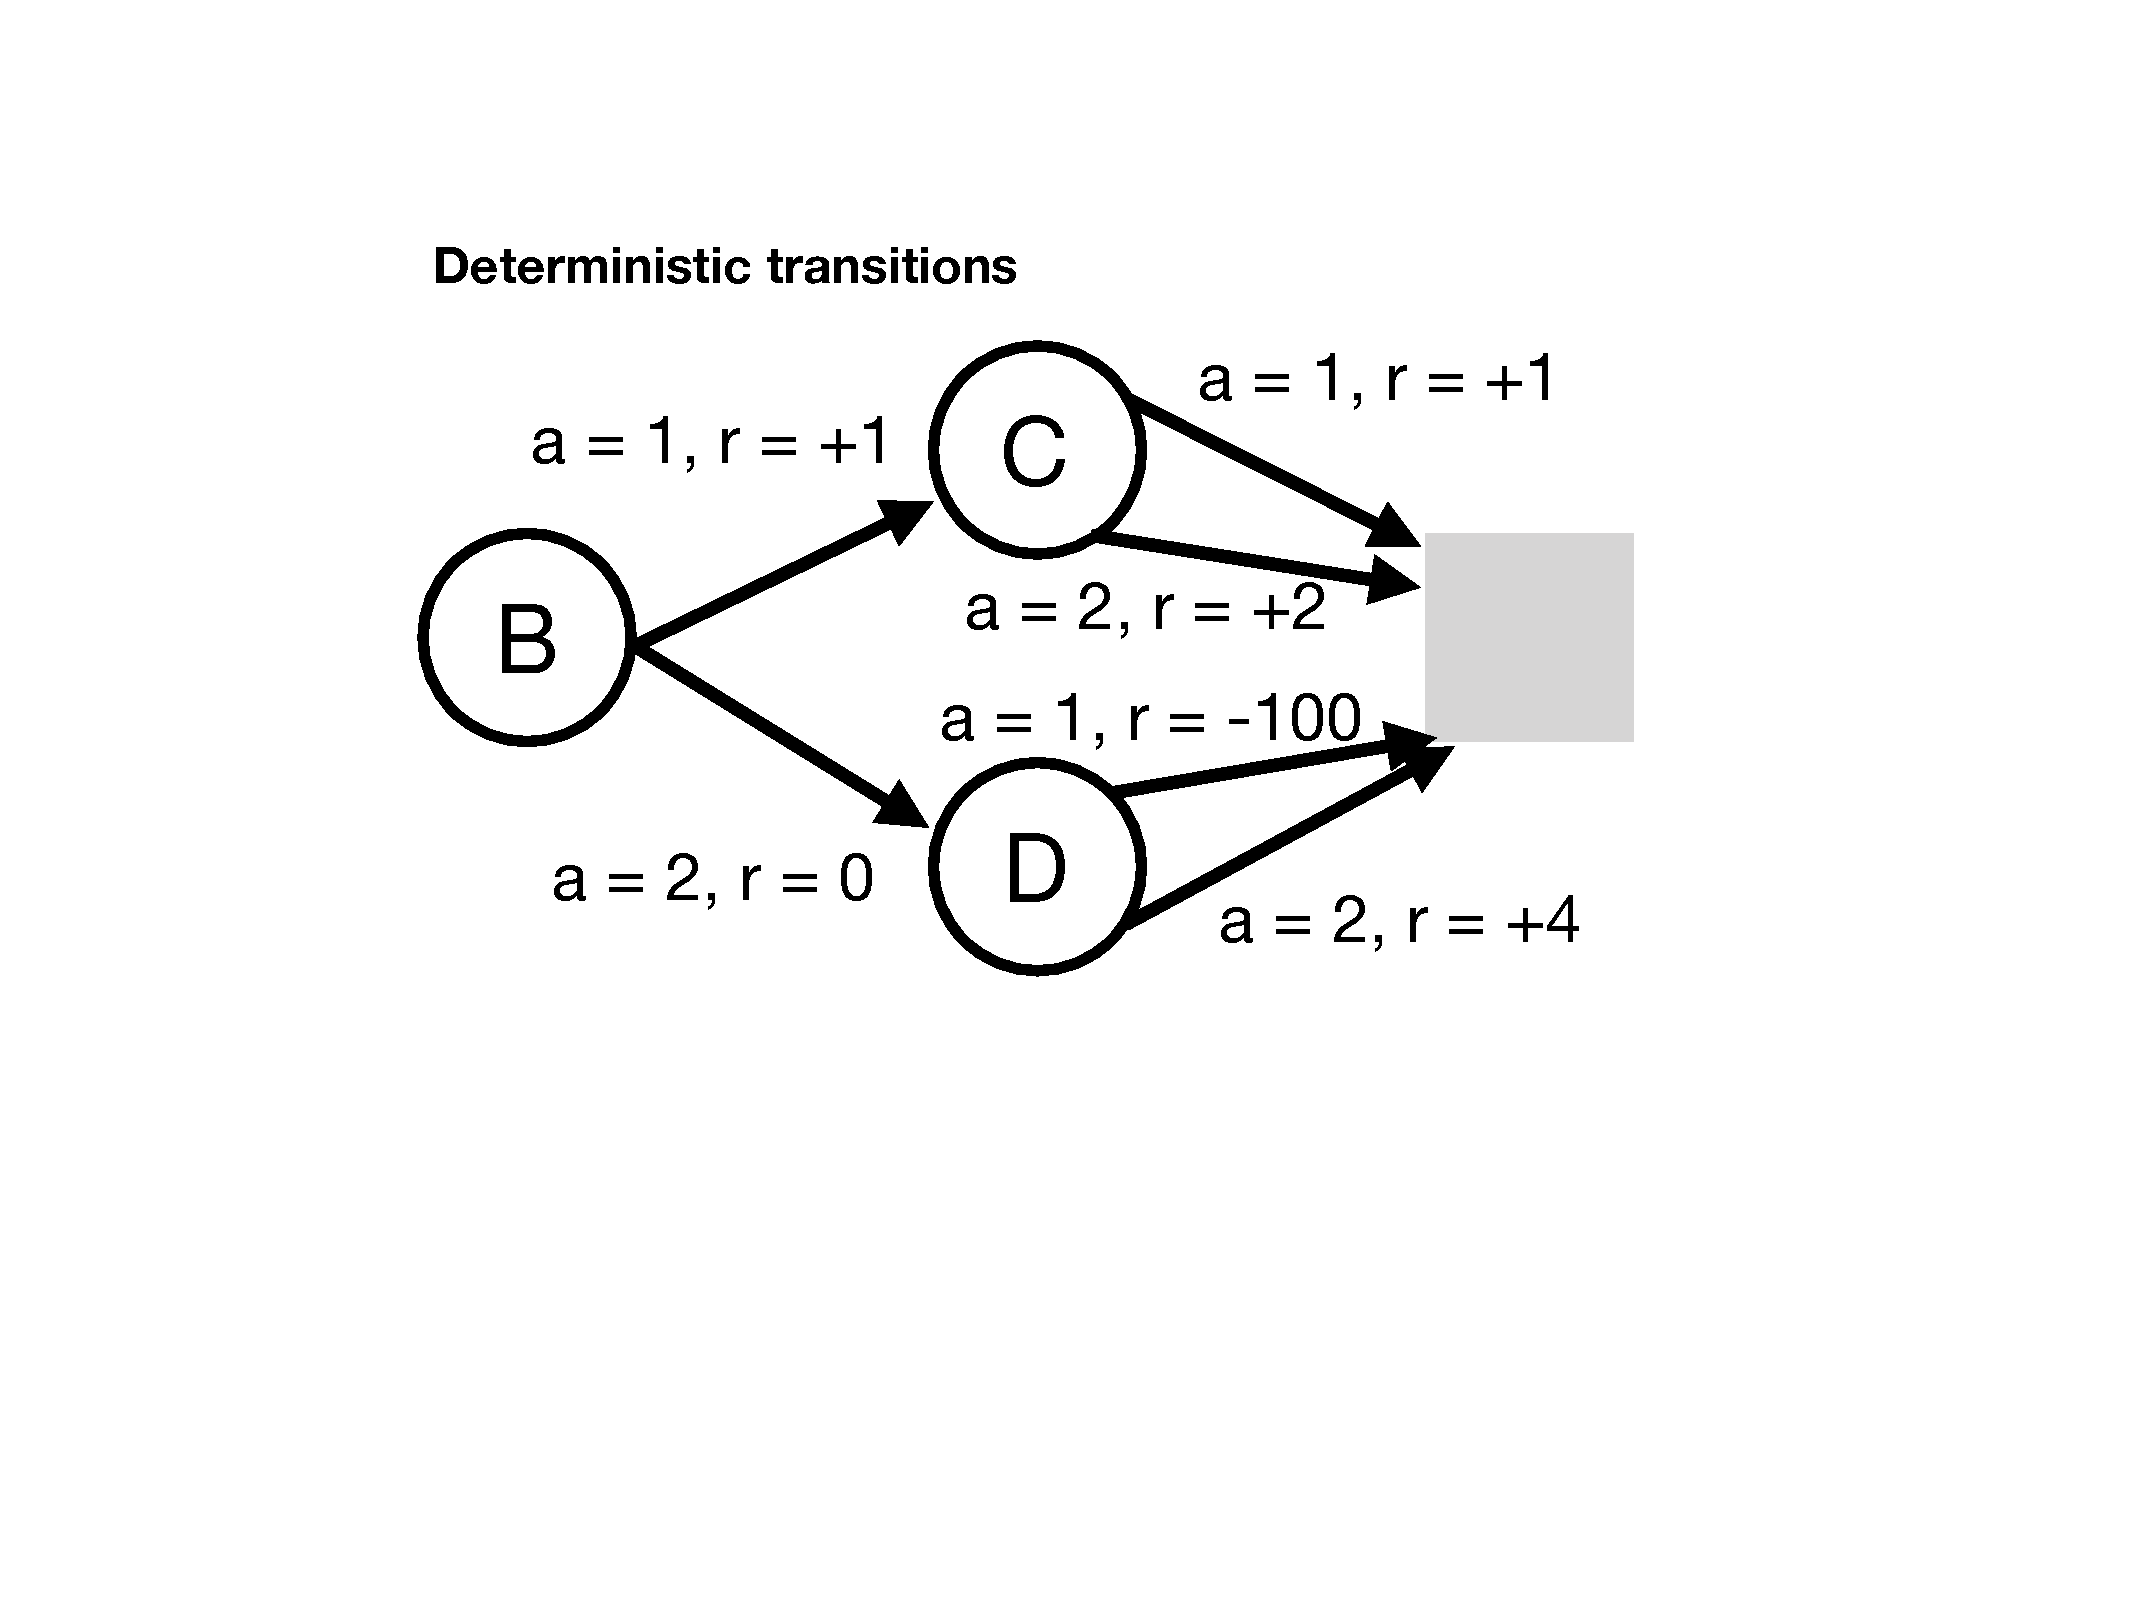
\includegraphics[width=0.5\linewidth]{figures/bcd.pdf}
\end{figure}

\subsubsection*{Answer:}
\begin{enumerate}
\item The Bellman equation for the optimal action value function is $q_*(s, a) = \sum_{s', r} p(s', r|s, a)[r + \gamma \max_{a'} q_*(s', a')]$. Using this, we obtain $q_*(C, 1) = 1, q_*(C, 2) = 2, q_*(D, 1) = -100, q_*(D, 2) = 4, q_*(B, 1) = 1+q_*(C, 2) = 3, q_*(B, 2) = 0+q_*(D, 2) = 4$. The optimal policy is greedy with respect to this value function. So, $\pi_*(2|C) = 1, \pi_*(2|D) = 1, \pi_*(2|B) = 1$ and zero for all other state action pairs.
\item  \textbf{SARSA:}

  $q(B, 2) = q(B, 2) + 0.1 [0 + \gamma q(D, 2) - q(B, 2)] = 0 + 0.1[0 + 0-0] = 0$, and

  $q(D, 2) = q(D, 2) + 0.1 [4 + \gamma q(T, \cdot) - q(D, 2)] = 0 + 0.1[4 + 0-0] = 0.4$.
  
\item\textbf{Q--learning:}

  $q(B, 2) = q(B, 2) + 0.1 [0 + \gamma \max_{a'} q(D, a') - q(B, 2)] = 0 + 0.1[0 + 0 - 0] = 0$ and

  $q(D, 2) = q(D, 2) + 0.1 [4 + \gamma \max_{a'} q(T, a') - q(D, 2)] = 0 + 0.1[4 + 0 - 0] = 0.4$.
  
\item
  \textbf{SARSA:}
  
  $q(B, 2) = q(B, 2) + 0.1 [0 + \gamma q(D, 1) - q(B, 2)] = 0 + 0.1[0 + 0-0] = 0$, and

  $q(D, 1) = q(D, 1) + 0.1 [-100 + \gamma q(T, \cdot) - q(D, 1)] = 0 + 0.1[-100  +0-0] = -10$.

  \textbf{Q--learning:}

  $q(B, 2) = q(B, 2) + 0.1 [0 + \gamma \max_{a'} q(D, a') - q(B, 2)] = 0 + 0.1[0 + 0.4 - 0] = 0.04$ and

  $q(D, 1) = q(D, 1) + 0.1 [-100 + \gamma \max_{a'} q(T, a') - q(D, 1)] = 0 + 0.1[-100 + 0 - 0] = -10$.
  
  
\item
    \textbf{SARSA:}
  
  $q(B, 2) = q(B, 2) + 0.1 [0 + \gamma q(D, 1) - q(B, 2)] = 0 + 0.1[0 + -10 -0] = -1$, and

  $q(D, 1) = q(D, 1) + 0.1 [-100 + \gamma q(T, \cdot) - q(D, 1)] = -10 + 0.1[-100  +0+10] = -19$.

  \textbf{Q--learning:}

  $q(B, 2) = q(B, 2) + 0.1 [0 + \gamma \max_{a'} q(D, a') - q(B, 2)] = 0.04 + 0.1[0 + 0.4 - 0.04] = 0.076$ and

  $q(D, 1) = q(D, 1) + 0.1 [-100 + \gamma \max_{a'} q(T, a') - q(D, 1)] = -10 + 0.1[-100 + 0 + 10] = -19$.

  We observe that the SARSA and Q--learning updates are same for $q(D, 1)$, and they are different for $q(B, 2)$. For $q(B, 2)$, Q--learning makes the update using the next state action pair as $q(D, 2)$ since it has a higher value than the other action value $q(D, 1)$.

\item Q--learning converges to the optimal greedy policy. Sarsa converges to the optimal policy in behavior policy class (for example the optimal $\epsilon$--greedy policy). The Cliff Grid World illustrates this.
\end{enumerate}

%% \subsubsection*{Q8}
%% Consider the following MDP, with two states $B$ and $C$, with 1 action in state $B$ and two actions in state $C$, with $\gamma = 1.0$.
%% Assume the action values are initialized, for all state-action pairs, $Q(s,a) = 0$.
%% \begin{enumerate}
%% \item What is the optimal policy for this MDP and what are the optimal action-values $q^{*}(s,a)$?
%% \item What policy is executed by being greedy with the initialized action-values?
%% \item Imagine you got to interact with the environment for one episode, and observed the episode $\{S_0 = B, A_0 = 1, R_1 = 1, S_1 = C, A_1 = 1, R_2 = 1$. This episode consists of two transitions, what is the SARSA update for both transitions?
%% \item For the transitions in the previous question, what is the Q-learning update?
%% \item If you see the same transitions again, how will the update change for SARSA and for Q-learning?
%% \end{enumerate}
%% \begin{figure}[h!]
%%   \center
%% 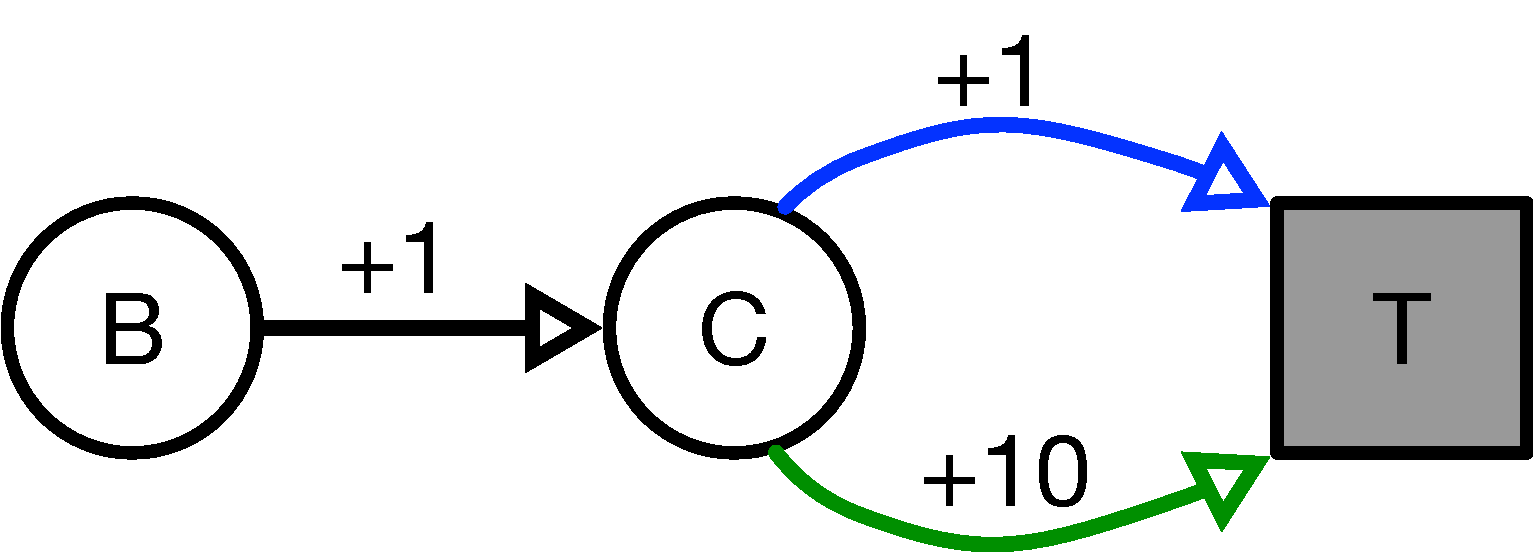
\includegraphics[width=0.5\linewidth]{figures/c2_2state.pdf}
%% \end{figure}
%% \subsubsection*{Answer:}

\subsubsection*{Q8}
In this question we compare the variance of the target for Sarsa and Expected Sarsa. Recall the update for Sarsa is 
$$ Q(S_{t}, A_{t}) \leftarrow Q(S_{t}, A_{t}) + \alpha \left[  R_{t+1} + \gamma Q(S_{t+1}, A_{t+1}) - Q(S_{t}, A_{t})\right]$$
and for Expected Sarsa is
$$ Q(S_{t}, A_{t}) \leftarrow Q(S_{t}, A_{t}) + \alpha \left[  R_{t+1} + \gamma \sum_{a' \in \mathcal{A}} \pi(a' | S_{t+1}) Q(S_{t+1}, a')  - Q(S_{t}, A_{t})\right].$$
\begin{enumerate}
\item Start by comparing the part of the update that is different: $Q(S_{t+1}, A_{t+1})$ compared to $\sum_{a' \in \mathcal{A}} \pi(a' | S_{t+1}) Q(S_{t+1}, a') $. Write down the variance for these two terms, given $S_{t+1} = s'$.
%
\begin{equation*}
\text{Var}(Q(s', A_{t+1})) \hspace{0.5cm} \text{ and }  \hspace{0.5cm}
\text{Var}\left(\sum_{a' \in \mathcal{A}} \pi(a' | s')Q(s', a')\right)
\end{equation*}
%
Conclude that the variance is zero for Expected Sarsa, but likely non-zero for Sarsa. Notice that the only random variable is $A_{t+1}$, which is the action selected according to the target policy $\pi$ with distribution $\pi(\cdot | S_{t+1})$. 
\item \textbf{Challenge Question:} Show that the variance of the Sarsa target is always greater than or equal to the variance of the Expected Sarsa target, given $S_t = s$ and $A_t = a$. Hint: use the law of total variance.
\end{enumerate}

\subsubsection*{Answer:}

\end{document}
